\documentclass{beamer}
\usepackage{beamerThemeLogic}
% \usetheme{Warsaw}
\usetheme{IrvineMath}

\usepackage{amsmath, amssymb}
\usepackage{physics}
\usepackage{svg}
\usepackage{mathtools}

\usepackage{graphicx}
\graphicspath{{../figures/}}

\usepackage{tikz}
\usetikzlibrary{arrows.meta}
\usetikzlibrary{calc}
\usetikzlibrary{decorations.markings}

\author{Eli Griffiths}
\title{A Spectral Approach To Meshes}
\institute[UCI]{University of California, Irvine}
\date{\today}

\directlua{graph = require("../scripts/graph")}
\directlua{examples = require("../scripts/data")}

\begin{document}

\maketitle

\begin{frame}{The Journey}
    \tableofcontents
\end{frame}

\section{Basics of Graphs}

\begin{frame}{The Graph Structure}
    \begin{definition}[Graph]
        A graph is a pair $G = (V, E)$ where $E$ is comprised of two element subsets of $V$. The elements of $V$ are called \emph{vertices} and the elements of $E$ \emph{edges}
    \end{definition}
    \pause
    \begin{center}
    \begin{tikzpicture}[
        scale=0.6,
        vertex/.style={
            font = \scriptsize,
            fill=blue!20,
            draw,
            circle,
            inner sep=0pt,
            minimum size=20pt,
        },
        edge/.style={}
    ]
        \directlua{graph.graph_tikz(examples.example1)}
    \end{tikzpicture}
    \end{center}
\end{frame}

\begin{frame}{Graphs $\Leftrightarrow$ Connectivity}
    Graphs at their core encode connectivity
    \begin{itemize}
        \item<2-> Friend networks on social media platforms
        \item<3-> Molecules and bonds between atoms in structural chemistry
        \item<4-> Connectivity of meshes in computational geometry
    \end{itemize}
    \only<4>{

    \begin{figure}
        \centering
        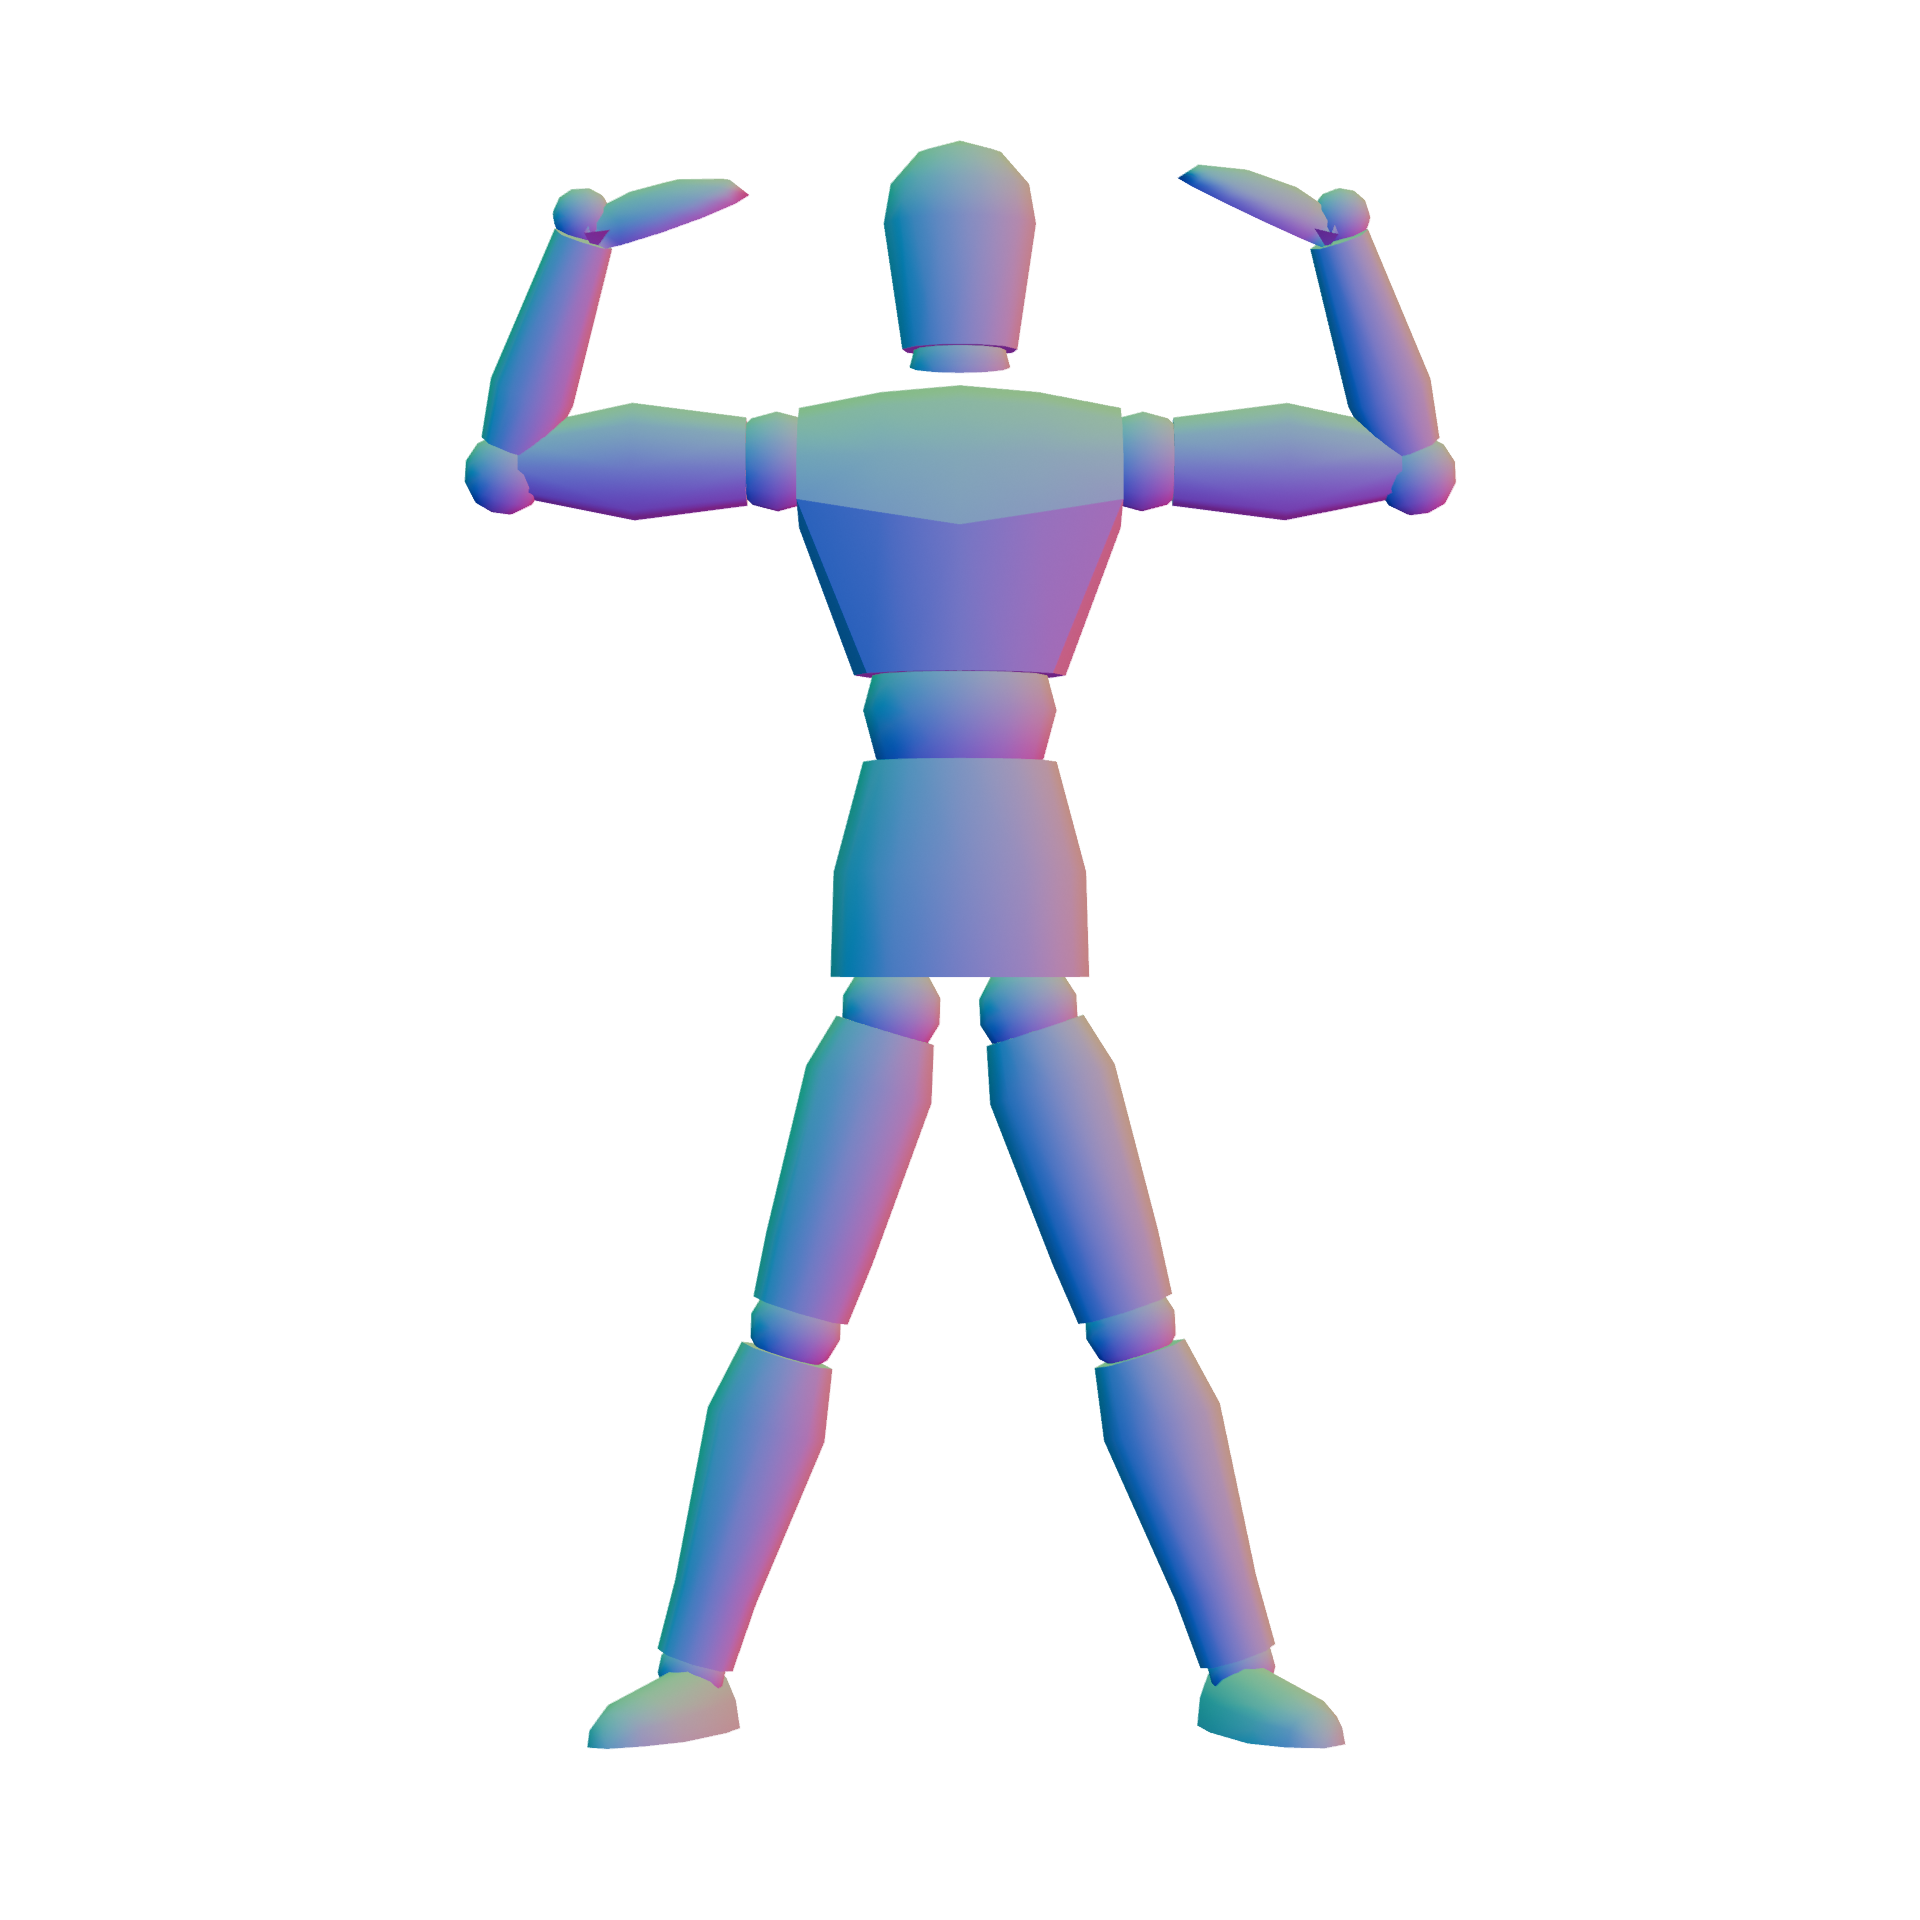
\includegraphics[width=0.3\textwidth]{figurine.png}
        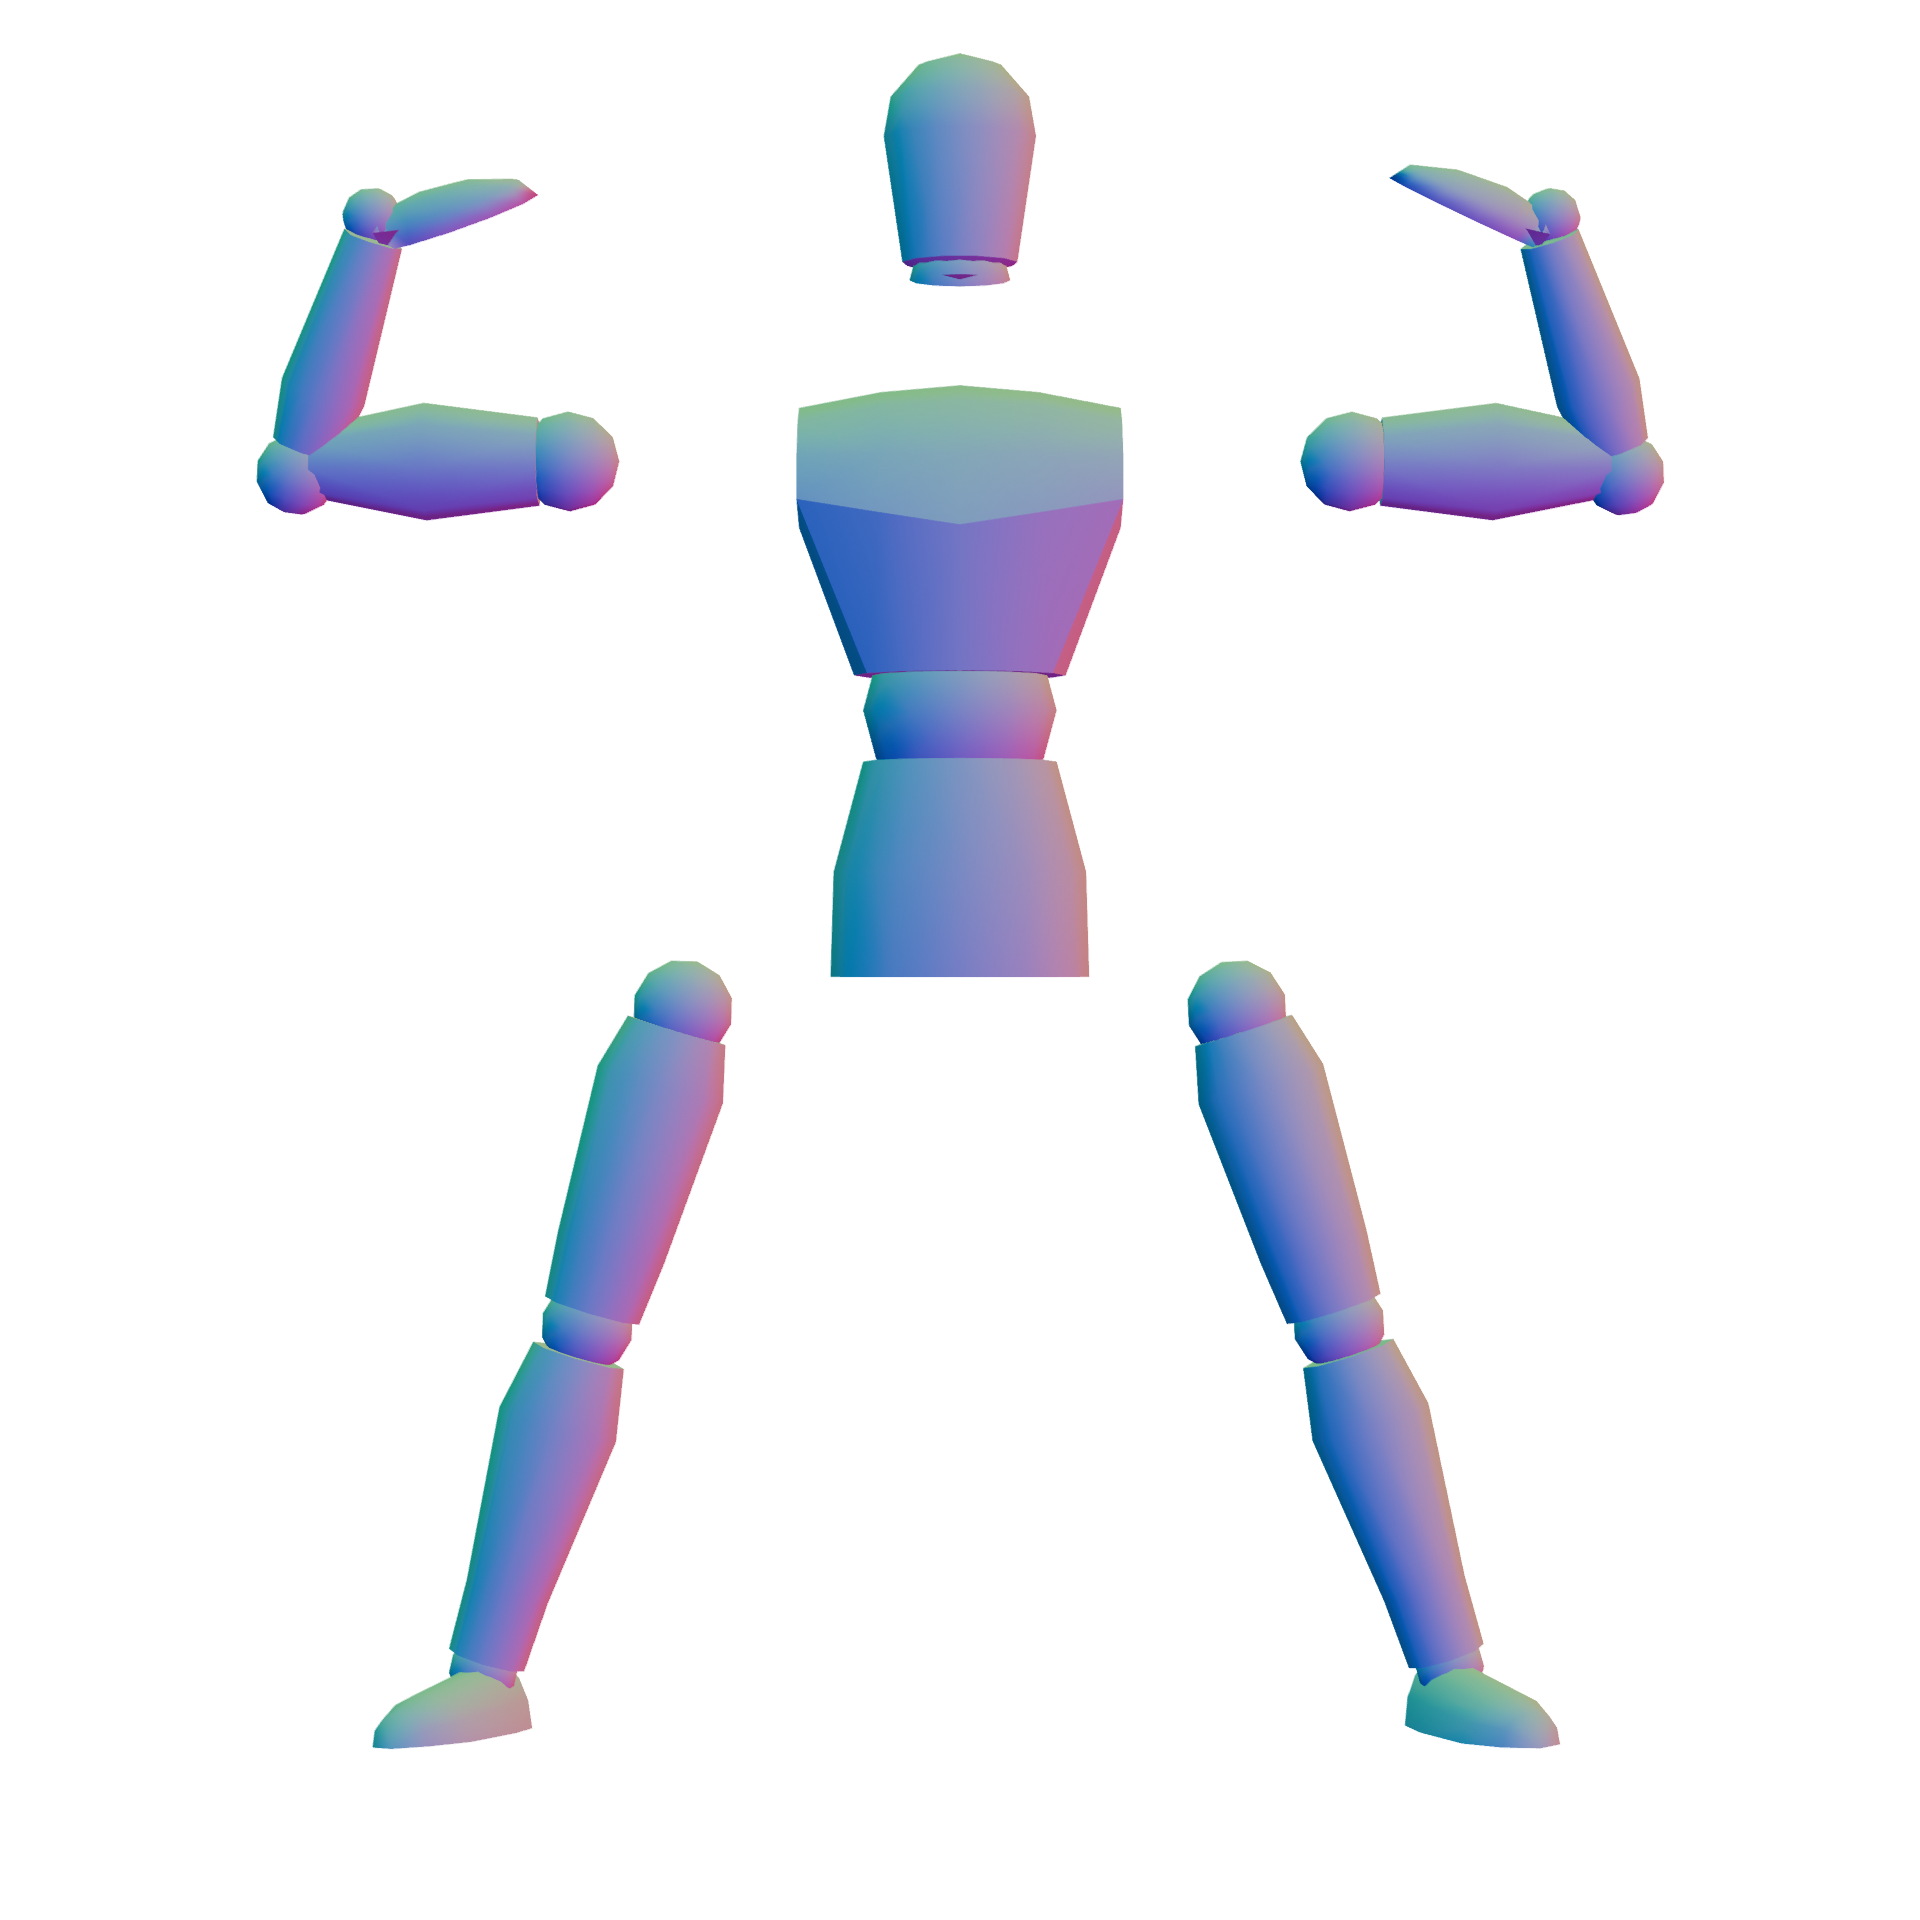
\includegraphics[width=0.3\textwidth]{figurine_split.png}
    \end{figure}
    }
\end{frame}

\begin{frame}
    \begin{center}
        \includesvg[width=0.6\pagewidth]{overlayed.svg}
    \end{center}
\end{frame}

\begin{frame}
    \begin{columns}
        \begin{column}{0.5\pagewidth}
            \begin{figure}[t]
                \centering
                \includesvg[width=0.9\textwidth]{overlayed_g1.svg}
            \end{figure}
        \end{column}
        \begin{column}{0.5\pagewidth}
            \begin{figure}[t]
                \centering
                \includesvg[width=0.9\textwidth]{overlayed_g2.svg}
            \end{figure}
        \end{column}
    \end{columns}
\end{frame}

\section{Matrix Representations}

\begin{frame}{Matrix Representations}
    \begin{center}
    \begin{tikzpicture}
        \onslide<1>{
        \matrix[
            nodes={draw, minimum size = 0.6cm},
            column sep=-\pgflinewidth,
            row sep=-\pgflinewidth
        ] (m1) {
            \directlua{graph.adj_grid_tikz(examples.example1, false)}
        };
        }

        \onslide<2->{
        \matrix[
            nodes={draw, minimum size = 0.6cm},
            column sep=-\pgflinewidth,
            row sep=-\pgflinewidth
        ] (m1) {
            \directlua{graph.adj_grid_tikz(examples.example1, true)}
        };
        }

        \onslide<1,2>{
            \begin{scope}[
                anchor=west,
                shift=(m1.east),
                yshift=-1cm,
                xshift=0.8cm,
                scale=0.5,
                vertex/.style={
                    font = \scriptsize,
                    fill=blue!20,
                    draw,
                    circle,
                    inner sep=0pt,
                    minimum size=20pt,
                },
                edge/.style={}
            ]
                \directlua{graph.graph_tikz(examples.example1)}
            \end{scope}
        }

        \onslide<3>{
            \draw[->, thick] ($(m1.east) + (0.05,0)$) -- ++(1,0);
            \node[anchor=west] (adj) at ($(m1.east) + (1,0)$) {$
            \begin{pmatrix}
                \directlua{graph.adj_matrix(examples.example1)}
            \end{pmatrix}
            $};
            \node[anchor=north] at (adj.south) {Adjacency Matrix $A$};
        }
    \end{tikzpicture}
    \end{center}
\end{frame}

\begin{frame}
    \begin{definition}[Degree Matrix]
        The degree matrix of a graph $G$ with $n$ vertices is the $n \times n$ matrix $D$ such that
        \[
            (D)_{ij} = \begin{cases}
                \deg(v_i) & i = j \\
                0 & i \neq j
            \end{cases}
        .\]
    \end{definition}

    \begin{definition}[Laplacian Matrix]
        The Laplacian matrix of a graph $G$ is
        \[
            L \coloneq D - A
        .\]
    \end{definition}

\end{frame}

\begin{frame}
    \begin{theorem}
        A graph has $m$ connected components if and only if zero has algebraic multiplicty $m$ for $L$
    \end{theorem}
    \begin{theorem}
        The eigenvector associated with the smallest positive eigenvalue of $L$ (called the ``Fiedler Vector'') defines a well behaved partitioning scheme of a graph.
    \end{theorem}
\end{frame}

\section{Computational Geometry}

\begin{frame}{Triangular Mesh}
    \begin{columns}
    \begin{column}{0.5\pagewidth}
        \begin{definition}[Triangular Mesh]
            A \textbf{triangular mesh} is a triple $K = (V, E, F)$ such that
            \begin{itemize}
                \item<2-> $V \subseteq \mathbb{R}^3$ is the set of vertices
                \item<3-> $E \subseteq [V]^2$ is the set of representing non-intersecting edges
                \item<4-> $F \subseteq [E]^3$ is the set of faces such that for any $f = \qty{e_1, e_2, e_3} \in F$, 
                    \begin{align*}
                        e_1 \cap e_2 &= \qty{v_1} \\
                        e_2 \cap e_3 &= \qty{v_2} \\
                        e_3 \cap e_1 &= \qty{v_3}
                    \end{align*}
                    for $v_1 \neq v_2 \neq v_3$. 
            \end{itemize}
        \end{definition}
    \end{column}

    \begin{column}{0.3\pagewidth}
        \begin{figure}
            \centering
            \only<1>{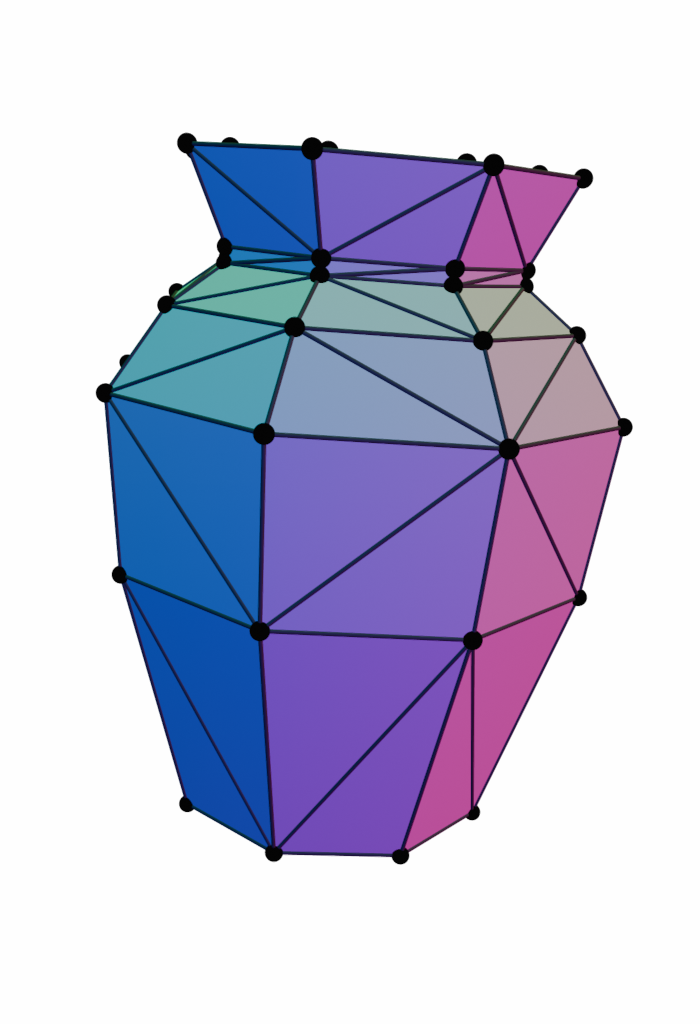
\includegraphics[width=0.3\pagewidth]{vase_all.png}}
            \only<2>{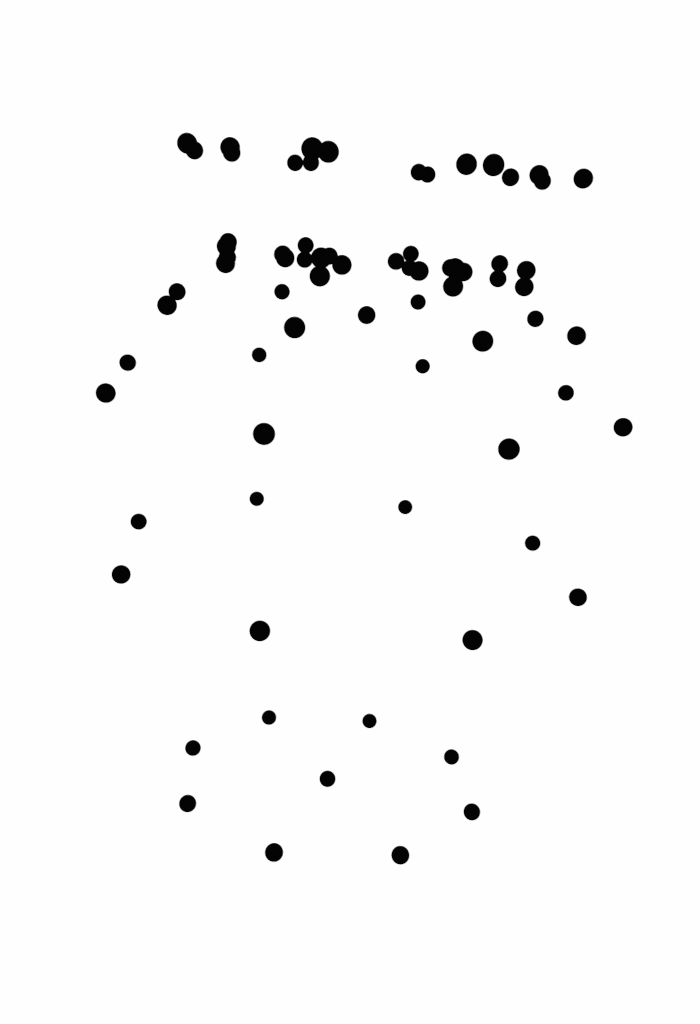
\includegraphics[width=0.3\pagewidth]{vase_vertices.png}}
            \only<3>{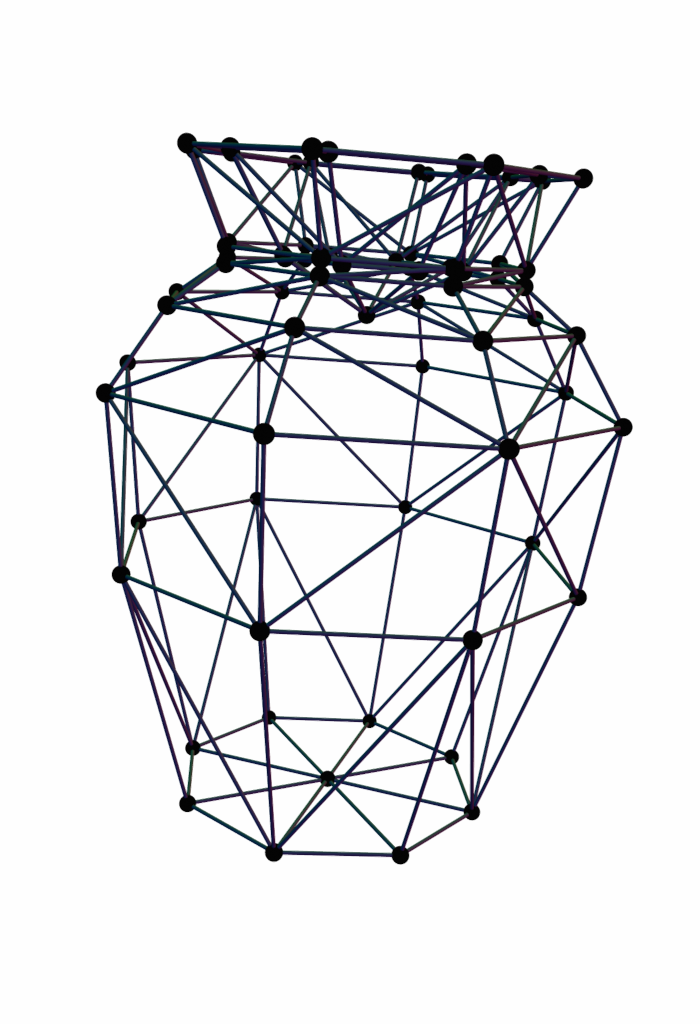
\includegraphics[width=0.3\pagewidth]{vase_edges.png}}
            \only<4>{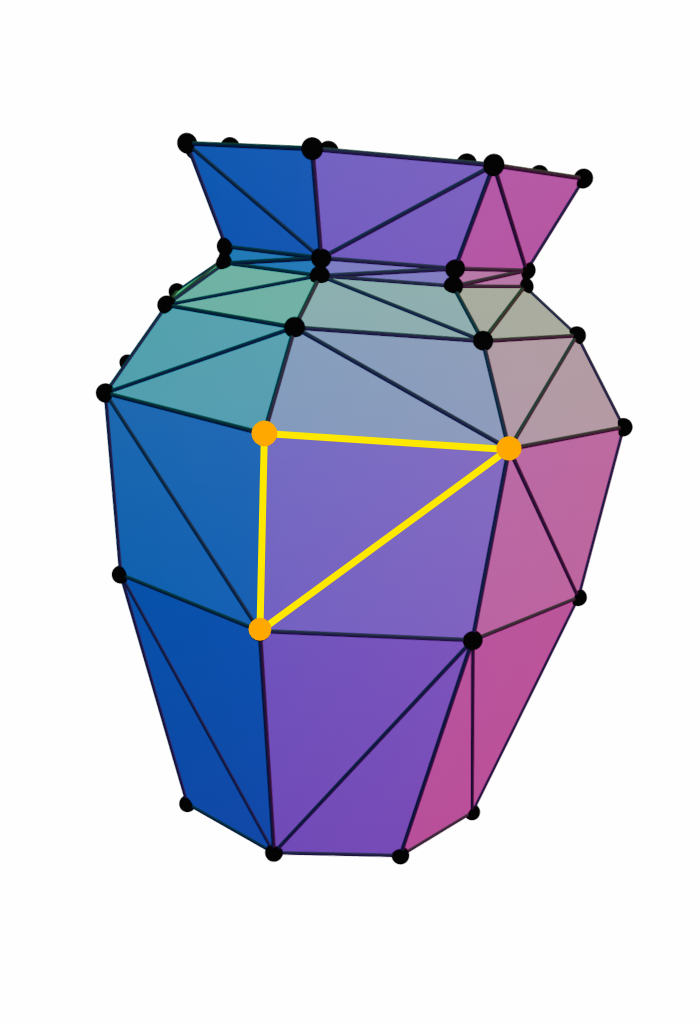
\includegraphics[width=0.3\pagewidth]{vase_face_highlight.png}}
        \end{figure}
    \end{column}
    \end{columns}
\end{frame}

\begin{frame}{Dual Mesh}
    \begin{figure}
        \centering
        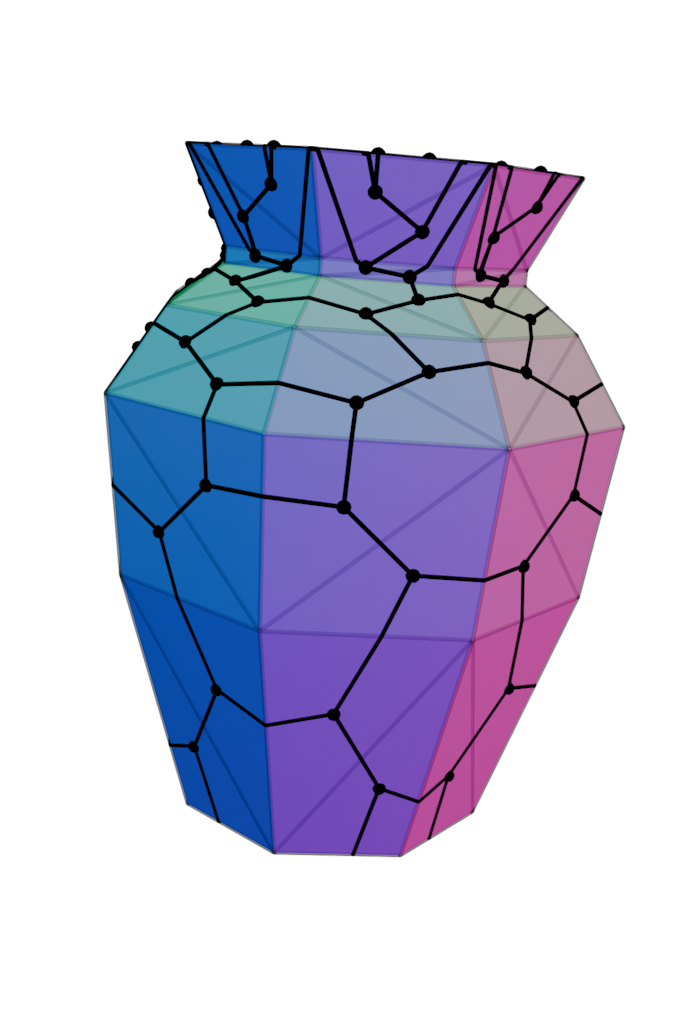
\includegraphics[width=0.3\textwidth]{vase_dual.png}
    \end{figure}
\end{frame}

\begin{frame}{Spectral Partitioning}
    \begin{columns}
        \begin{column}{0.3\pagewidth}
            \begin{figure}
                \centering
                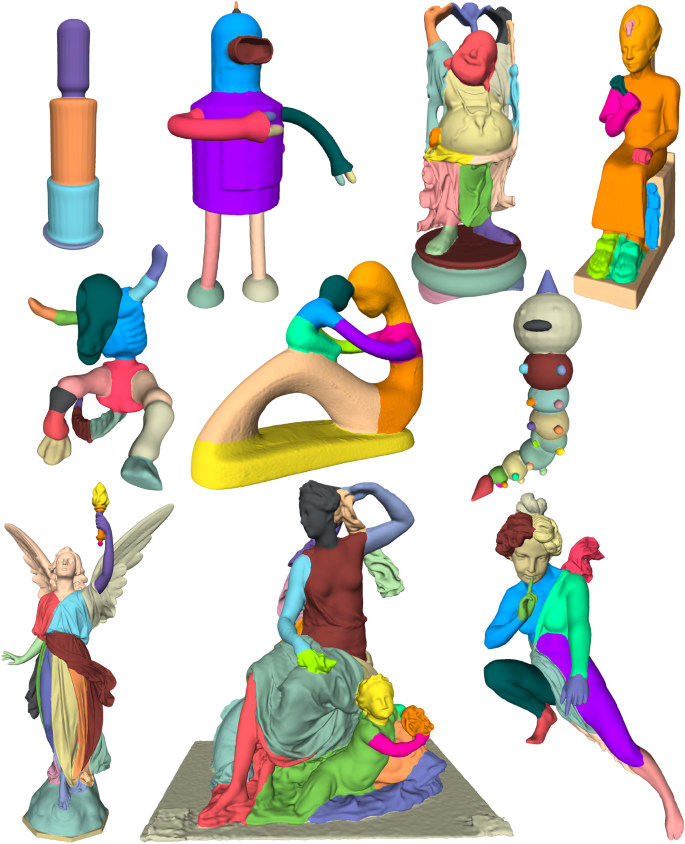
\includegraphics[width=\textwidth]{spectral_partitioning.png}
            \end{figure}
        \end{column}
        \begin{column}{0.5\pagewidth}
            \begin{figure}
                \centering
                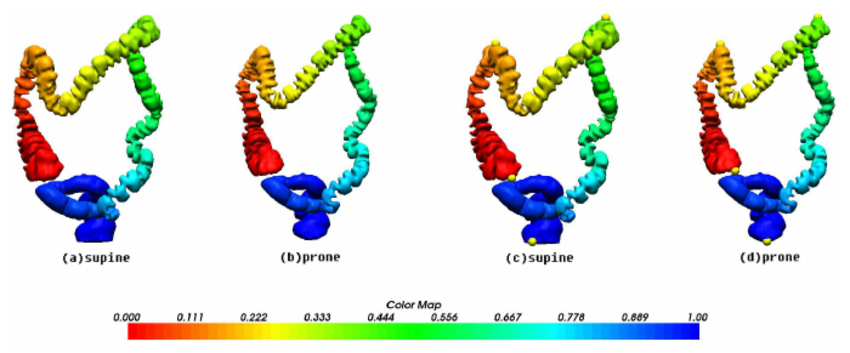
\includegraphics[width=\textwidth]{fielder_vector_colon.png}
            \end{figure}
        \end{column}
    \end{columns}
\end{frame}
    
\end{document}
